\documentclass{notes}

\usepackage[bb=boondox]{mathalfa} % чтобы делать двойные цифры

\author{\sffamily{\Large{Михаил Пирогов}} \\ \sffamily{\Large{записал со слов лектора А. А. Лодкина}}}
\title{\sffamily{\Huge{Анализ, 4 семестр}}}

\DeclareMathOperator{\Cell}{Cell}

\begin{document}
	\maketitle
\chapter{Теория меры}

\section{Алгебры и \texorpdfstring{$\sigma$}{σ}-алгебры множеств.}

	\begin{de}
		Пусть $X$~--- некоторое множество. Тогда $\mc{A} \subset 2^{X}$ называется \ti{алгеброй,} если выполняются следующие условия:
		\begin{enumerate}
			\item $\varnothing, \, X \in \mc{A},$
			\item $A, \, B \in \mc{A} \so A \cup B, \, A \cap B, \, A \setminus B \in \mc{A}.$
		\end{enumerate} 
	\end{de}

	\begin{exc}
		Пусть $\mc{A} \subset 2^X$~--- алгебра, $|\mc{A}| < \infty$. Тогда $|\mc{A}| = 2^n$ для некоторого $n$.
		\begin{proof}
			Так как $X \in \mc{A},$ каждый элемент $X$ содержится как минимум в одном элементе $\mc{A}$. Пусть $A(x)$~--- пересечение всех множеств из $\mc{A},$ содержащих $x$. Понятно, что $A(x)$ непусто, т.к. $x \in A(x)$. Разобьём дальнейшее доказательство на несколько пунктов:
			\begin{enumerate}
				\item Мы определили $A(x),$ как наименьшее по включению множество, удовлетворяющее некоторому свойству. Поэтому у него есть эквивалентное определение: $A(x)$~--- такое множество, что если $x \in B \in \mc{A},$ то $A(x) \subset B$ \footnote{Заметим, что мы существенно испльзуем конечность $\mc{A}$ каждый раз, когда говорим, что $A(x) \in \mc{A}$!}.
				\item Введём отношение на $X\col$ пусть $x \sim y,$ если $A(x) = A(y)$. Очевидно, что это отношение эквивалентности. Докажем, что $x \sim y \eqv y \in A(x)$.

				Пусть $y \in A(x)$. Предположим, что $A(y) \neq A(x)$. Тогда выполняется минимум одно из двух утверждений: либо $A(y)$ содержит элемент, которого нет в $A(x),$ либо наоборот. Пусть первое. Тогда $B = A(x) \cap A(y)$~--- элемент $\mc{A},$ который содержит $y$ и строго меньше $A(y),$ чего не может быть. Пусть второе. Тогда если $A(y)$ не содержит $x,$ то $A(x) \setminus A(y)$ является элементом $\mc{A},$ содержащим $x,$ а если содержит, то снова $A(x) \cap A(y)$ является таким элементом. Причём строго меньшим, чем $A(x),$ что опять ведёт нас к противоречию.

				Пусть $A(x) = A(y)$. Предположим, что $y \notin A(x)$. Но тогда $y \notin A(y),$ что точно ложь.
				\item Разобьём $X$ на классы эквивалентности по отношению $\sim\scol$ обозначим множество этих классов $\hat{\mc{A}}$. Понятно, что $|\hat{\mc{A}}| < \infty,$ ведь $\hat{\mc{A}} \subset \mc{A}$. Пусть $B \in \mc{A}$ и $\hat{B} \in \hat{\mc{B}}$. Докажем, что если $B \cap \hat{B} \neq \varnothing,$ то $B \cap \hat{B} = \hat{B}$.

				Предположим противное: пусть $x \in B \cap \hat{B}$ и $y \in \hat{B} \setminus B$. Из определения отношения эквивалентности понятно, что $\hat{B} = A(x) = A(y)$. Но заметим тогда, что $\hat{B} \setminus B$~--- множество из $\mc{A},$ содержащее $y$ и строго меньшее $\hat{B},$ чего не может быть.
				\item Из сделанного нетрудно увидеть, что любое $B \in \mc{A}$ можно представить, как объединение множеств из $\hat{\mc{A}}\col$ просто для каждого $b \in B$ взять $A(b)$ и объединить их все. При этом понятно, что любое объединение множеств из $\hat{\mc{A}}$ лежит в $A$. Т.к. элементы $\hat{\mc{A}}$ не пересекаются, нетрудно увидеть, что отображение, сопоставляющее множеству $\mc{B} \subset \hat{\mc{A}}$ объединение всех его элементов есть биекция~--- биекция между множествами $2^{\hat{\mc{A}}}$ и $\mc{A}$. Поэтому количество элементов $\mc{A}$ имеет искомый вид.
			\end{enumerate}
		\end{proof}
	\end{exc}

	Примеры привести не очень сложно, не будем здесь на этом останавливаться.

	\begin{de}
		\ti{$\sigma$-алгеброй} называется алгебра, замкнутая относительно счётных объединений и пересечений.
	\end{de}

	\begin{de}
		Пусть $\mc{E} \subset 2^X.$ Тогда наименьншая $\sigma$-алгебра, содержащая $\mc{E},$ называется \ti{борелевской оболочкой} $\mc{E}$ и обозначается $\sigma(\mc{E})$. (Ссылаясь на факт, который уже упоминался в упражнении, заметим, что $\sigma(\mc{E})$ совпадает с пересечением всех $\sigma$-алгебр, содержащих $E$).
	\end{de}

	\begin{lm}
		Если $\mc{E}_2 \subset \sigma(\mc{E}_1),$ то $\sigma(\mc{E}_2) \subset \sigma(\mc{E}_1)$.
		\begin{proof}
			Из определения борелевской оболочки понятно, что 
			\[
				\mc{E}_2 \subset \sigma(\mc{E}_1) \so \sigma(\mc{E}_2) \subset \sigma(\sigma(\mc{E}_1)).
			\]
			При этом понятно, что правая часть равна $\sigma(\mc{E}_1),$ чего нам и надо.
		\end{proof}
	\end{lm}

\section{Борелевская \texorpdfstring{$\sigma$}{σ}-алгебра.}

	\begin{de}
		Пусть $\mc{O}_n$~--- множество всех открытых множеств в $\R^n$. Тогда $\sigma$-алгебра $\sigma(\mc{O}_n)$ называется \ti{борелевской}.
	\end{de}

	\begin{de}
		Назовём \ti{$n$-мерной ячейкой} такое подмножество $\R^n\col$
		\begin{align*}
			n &= 1 \so \Delta = \begin{cases}
				[a, \, b), \; [a, \, \infty)\scol \\
				(-\infty, \, b), \; (-\infty, \, \infty)\scol 
			\end{cases} \\
			n &> 1 \so \Delta = \prod_{i = 1}^k \Delta_i,
		\end{align*}
		где $\Delta_i$~--- одномерные ячейки.
	\end{de}

	\begin{de}
		Назовём \ti{$n$-мерной алгеброй ячеек} множество
		\[
			\Cell_n = \left\{\bigcup_{i = 1}^k \Delta_i \, \bigg| \, k \in \N \right\},
		\]
		где $\Delta_i$~--- ячейки.
	\end{de}

	\begin{st}
		$\Cell_n$~--- действительно алгебра.
		\begin{proof}
			Чтобы сделать, нужно увидеть, что пересечение ячеек~--- ячейка, а потом представить пересечение объединений, как объединение пересечений.
		\end{proof}
	\end{st}

	\begin{thm}
		$\sigma(\Cell_n) = \sigma(\mc{O}_n)$.
		\begin{proof}
			Зная последний результат из предыдущего билета, имеем возможность доказывать, что
			\[
				\Cell_n \subset \sigma(\mc{O}_n) \text{ и } \mc{O}_n \subset
				 \sigma(\Cell_n).
			\]
			Это даст нам утверждение теоремы.

			Первое включение очевидно: можно представить любую ячейку, как пересечение вложенных прямоугольников, например. Поэтому и с объединением проблем не будет.

			Чтобы доказать второе, рассмотрим сначала ячейки с целыми вершинами, назовём их ячейками первого ранга. Побив каждую из них на $2^n$ частей (поделив каждую сторону на 2), получим ячейки второго ранга, продолжая процесс~--- ячейки ранга $n$. Пусть $U$~--- произвольное открытое множество, а $U_k$--- объединение всех ячеек ранга $k,$ пересекающих $U$.

			Рассмотрим $x$~--- произвольную точку не из $U$. Т.к. $U$ открыто, существует такое $\varepsilon,$ что  \[
				B_{\varepsilon}(x) \cap U = \varnothing.
			\]
			Заметим однако, что если ячейка ранга $k,$ то её сторона равна $2^{1 - k},$ а значит, диагональ~---
			\[
				\sqrt{n} \, 2^{1 - k}.
			\]
			Эта последовательность стремится к нулю при $k$ стремящемся к бесконечности, поэтому можно сделать так, что диагональ ячейки станет меньше, чем $\varepsilon,$ при всех $k > K$. Из этого будет следовать, что при $k > K \; x \notin U_k$.

			Отсюда ясно, что
			\[
				U = \bigcap_{k = 1}^{\infty} U_k \so U \in \sigma(\Cell_n) \so \mc{O} \subset \sigma(\Cell_n). 
			\]
		\end{proof}
	\end{thm}

	\begin{st}
		Борелевской $\sigma$-алгебре принадлежат множества следующих типов:
		\begin{enumerate}
			\item Точки.
			\item Открытые, замкнутые.
			\item Не более чем счётные.
			\item Счётные пересечения открытых множеств~--- множества типа $G_{\delta}$.
			\item Счётные объединения замкнутых~--- множества типа $F_{\sigma}$.
			\item Счётные объединения множеств типа $G_{\delta}$~--- множества типа $G_{\delta \sigma}$.
			\item Счётные пересечения множеств типа $F_{\sigma}$~--- множества типа $F_{\sigma \delta}$.
		\end{enumerate}
	\end{st}

\section{Мера на алгебре. Примеры мер.}

	\begin{de}
		Пусть $X$~--- множество, $\mc{A}$~--- алгебра на $X$. Тогда \ti{мерой} на $\mc{A}$ называется отображение $\mu \col \; \mc{A} \to [0, \, \infty],$ удовлетворяющее двум свойствам:
		\begin{enumerate}
			\item $\mu(\varnothing) = 0.$
			\item Если $\{A_k\}_{k = 1}^{\infty}$~--- семейство дизъюнктных\footnote{Попарно непересекающихся друг с другом. Если в объединении участвует семейство дизъюнктных множеств, то будем его обозначать $\sqcup$ вместо $\cup,$ забывая упоминать дизъюнктность.} множеств из $\mc{A},$ то 
			\[
				\mu \left(\bigsqcup\limits_{k = 1}^{\infty} A_k\right) = \sum\limits_{k = 1}^{\infty} \mu(A_k).
			\]
		\end{enumerate}
	\end{de}

	\begin{exm}
		Пусть $\mc{A} = 2^{X}$, и $a \in X$~--- произвольная точка. Введём меру
		\[
			\mu(A) = \begin{cases}
				1, \; a \in A, \\
				0, \; a \notin A.
			\end{cases}
		\]
			\begin{proof}[Проверка аксиом]
				Первое свойство, конечно, выполняется; чтобы проверить второе, можно увидеть, что в семействе дизъюнктных множеств точка может содержаться лишь в одном из них. 
			\end{proof}
		Такая мера называется \ti{дельта-мерой, атомической мерой} или \ti{мерой Дирака,} обозначается, как $\delta_a$. В физике порой рассматривается (на $\R$), как интеграл от \ti{дельта-функции Дирака}~--- такой функции, что она равна нулю всюду, кроме $a,$ а интеграл по всей прямой от неё равен $1$.
	\end{exm}

	\begin{exm}
		В той же ситуации вместо точки $a$ зафиксируем не более, чем счётное множество точек $\{a_k\}$. Меру определим, как
		\[
			\mu(A) = \sum \limits_{k} m_k \delta_{a_k}(A),
		\]
		где $m_k$~--- некторые фиксированные неотрицательные вещественные числа, \ti{веса}. Такая мера называется\ti{молекулярной.}
		\begin{proof}[Проверка аксиом]
			Первая снова тривиальна, вторая следует из счётной аддитивности дельта-меры (на самом деле, тут нужно воспользоваться теоремой о перестановке/группировке членов в абсолютно сходящемся ряде; т.к. всё положительно, никакой условной сходимости тут не бывает, и при перестановке/группировке членов сохраняется как сходимость, так и расходимость).
		\end{proof}
	\end{exm}

	\begin{exm}
		В той же ситуации пусть
		\[
			\mu(A) = |A|.
		\]
	\end{exm}

\section{Свойства меры}
	
	\begin{pr}[Монотонность]
		Пусть $A, \, B \in \mc{A}, \; A \subset B$. Тогда $\mu(A) \leqslant \mu(B)$.
		\begin{proof}
			\[
				\mu(B) = \mu(A) + \mu(B \setminus A) \geqslant \mu(A).
			\]
		\end{proof}
	\end{pr}

	\begin{pr}
		Пусть $A, \, B \in \mc{A}, \; A \subset B, \; \mu{B} < \infty$. Тогда $\mu(B \setminus A) = \mu{B} - \mu{A}$.
		\begin{proof}
			\[
				\mu(B) = \mu(A) + \mu(B \setminus A) \so \mu(B \setminus A) = \mu(B) - \mu(A).
			\]
			Условие $\mu(B) < \infty$ было использовано, когда мы вычли $\mu(A)$ из двух частей равенства; действительно, по предыдущему свойству $\mu(A) \leqslant \mu(B) < \infty,$ поэтому $\mu(A)$ можно вычитать. \footnote{Не достаточно ли потребовать, что $\mu(A) < \infty$?}
		\end{proof}
	\end{pr}

	\begin{pr}[Усиленная монотонность]
		Пусть $A_1, \, ..., \, A_n, \, B \in \mc{A}, \; A_1, \, ..., \, A_n \subset B,$ причём множества $A_k$ дизъюнктные. Тогда 
		\[
			\sum\limits_{k = 1}^n \mu(A_k) \leqslant \mu(B).
		\] 
		\begin{proof}
			Очевидно.
		\end{proof}
	\end{pr}

	\begin{pr}[Полуаддитивность]
		Пусть $A_1, \, ..., \, A_n, \, B \in \mc{A}, \; B \subset \cup A_k$. Тогда
		\[
			\mu(B) \leqslant \sum\limits_{k = 1}^n \mu(A_k).
		\]
		\begin{proof}
			Введём семейство множеств:
			\[
				C_{k} = A_{k} \setminus \bigcup_{i = 1}^{k - 1} A_i, \; 1 \leqslant k \leqslant n.
			\]
			Нетрудно понять, что они дизъюнктны; при этом 
			\[
				\bigsqcup\limits_{k = 1}^n C_{k} = \cup A_k,
			\]
			потому что никаких точек извне $\cup A_k$ в это объединение точно попасть не может, а для любой точки $a$ из $\cup A_k$ можно взять наименьшее $k_0$ такое, что $a \in A_{k_0};$ тогда $a \in C_{k_0}$. 

			Из этого следует, что $B$ можно представить, как
			\[
				B = \bigsqcup \limits_{k = 1}^n B \cap C_k = \bigsqcup \limits_{k = 1}^n D_k.
			\]

			Заметим, что 
			\[
				\mu(D_k) = \mu(B \cap C_k) \leqslant \mu(C_k) \leqslant \mu(A_k).
			\]
			Поэтому и
			\[
				\mu(B) = \sum\limits_{k = 1}^n \mu(D_k) \leqslant \sum\limits_{k = 1}^n \mu(A_k).
			\]
		\end{proof}
	\end{pr}

	\begin{pr}[Непрерывность меры снизу]
		Пусть $\{A_k\}_{k = 1}^{\infty}$~--- такое семейство множеств из $\mc{A},$ что $A_k \subset A_{k + 1},$ и 
		\[
			A = \bigcup\limits_{k = 1}^{\infty} A_k \in \mc{A}.
		\]
		Тогда $\mu(A) = \lim \mu(A_k)$.
		\begin{proof}
			Пусть $C_k = A_{k} \setminus A_{k-1},$ причём $A_0 = \varnothing$ и $k \geqslant 1.$ Тогда нетрудно увидеть, что $C_k$ дизъюнктны, и
			\[
				A_k = \bigsqcup_{i = 1}^k C_k.
			\]
			При этом
			\[
				A = \bigsqcup_{i = 1}^{\infty} C_k.
			\]
			Но тогда искомое утверждение очевидно из второй аксиомы меры и определения суммы ряда.
		\end{proof}
	\end{pr}

	\begin{pr}[Непрерывность меры сверху]
		Пусть $\{A_k\}_{k = 1}^{\infty}$~--- такое семейство множеств из $\mc{A},$ что $A_k \supset A_{k + 1}, \; \mu A_1 < \infty$ и 
		\[
			B = \bigcap\limits_{k = 1}^{\infty} A_k \in \mc{A}.
		\]
		Тогда $\mu(B) = \lim \mu(A_k)$.
		\begin{proof}
			Пусть $B_k = A_{k-1} \setminus A_{k},$ причём $A_0 = \varnothing$ и $k \geqslant 1.$ Тогда нетрудно увидеть, что $B_k$ дизъюнктны, и
			\[
				A_k \sqcup \bigsqcup_{i = 1}^k B_k = A_1.
			\]
			При этом
			\[
				A \sqcup \bigsqcup_{i = 1}^{\infty} B_k = A_1.
			\]
			Конечность всех мер позволяет завершить доказательство так же, как в прошлый раз, перенеся суммы рядов вправо и перейдя к пределу.
		\end{proof}
	\end{pr}

	\begin{thm}
		Если мера конечно-аддитивна и непрерывна снизу (или сверху), то она счётно-аддитивна.
	\end{thm} 

\section{Объём в \texorpdfstring{$\R^n$}{𝐑n}. Мера Лебега и её свойства.}

	\begin{de}
		\ti{Объёмом} ячейки $\Delta = \sqcap \Delta_i$ в $\R^n$ называется
		\[
			v_n(\Delta) = \prod\limits_{i = 1}^n |\Delta_i|.
		\]
		Аналогично определим и объём открытых/замкнутых прямоугольников для удобства.
	\end{de}

	\begin{st}
		Любой элемент $\Cell_n$ можно представить, как дизъюнктное объединение ячеек (разбить на ячейки).
		\begin{proof}[Набросок доказательства]
			Кажется, делается двойной индукцией по количеству ячеек. Предполагаем сначала, что мы научились объединение $n$ прямоугольников представлять в виде дизъюнктного объединения нескольких ячеек. После этого делаем переход: доказываем, что если добавить $(n+1)$-ю ячейку, то всё равно получится.

			Чтобы доказать переход, вновь применяем индукцию. Предположим, что мы доказали, что можем представить в виде дизъюнктного объединения объединение ячейки и дизъюнктного объединения $k$ ячеек. А потом новый переход: добавляем $(k + 1)$-ю. Здесь удобно рассматривать <<сетчатую>> конструкцию разбиения: на пути индукции всё время поддерживать разбиение таким, чтобы все разрезающие линии кончались на границе какой-нибудь из объединяемых в данный момент ячеек.
		\end{proof}
	\end{st}

	\begin{de}
		\ti{Объёмом} элемента $\Cell_n$ называется сумма объёмов ячеек, входящих в его разбиение.
	\end{de}

	\begin{st}[Корректность]
		Объём элемента $\Cell_n$ не зависит от выбора разбиения.
		\begin{proof}[Набросок доказательства]
			Обсудим сначала случай $n = 2$. Проделаем с разбиением операции как на картинке, проверив, что объём в смысле нашего определения сохранится: 
			\begin{figure}[h]
				\begin{center}
					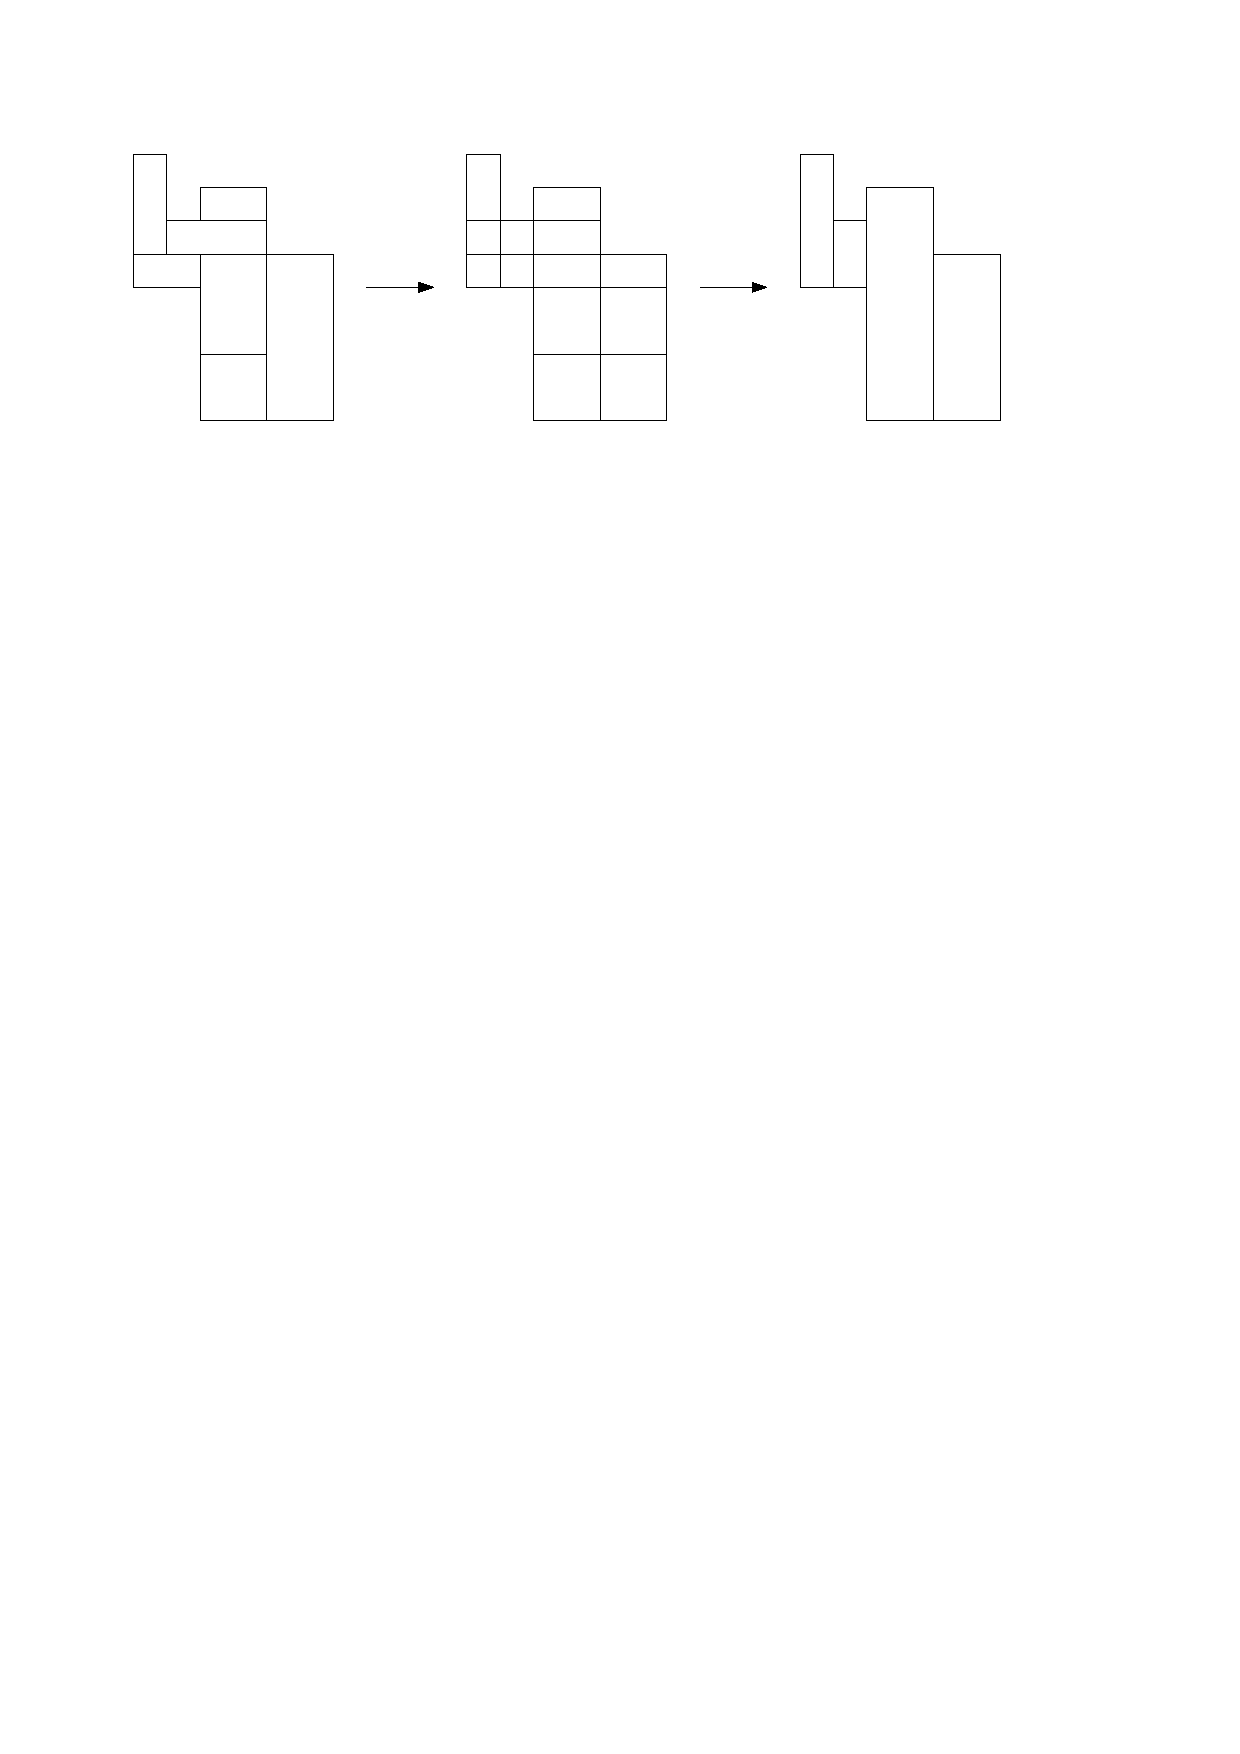
\includegraphics[scale = 0.5]{rects.pdf}
				\end{center}
			\end{figure}

			Если у нас было какое-то другое разбиение, мы получим какое-то другое разбиение на столбцы. После этого не очень трудно доказать, что два разбиения на столбцы задают одинкаовые объёмы: нужно просто нанести и те, и те линии, а после доказать, что <<суммарное>> разбиение задаёт тот же объём.

			В $n$-мерном случае нужно действовать индукцией по размерности: основания <<столбцов>> будут многомерные, а независимость от разбиения для $n-1$ будет использоваться, когда мы будем смотреть на разбиения оснований.
 		\end{proof}
	\end{st}

	\begin{thm}
		Объём~--- конечно-аддитивная функция на $\Cell_n$.
		\begin{proof}
			Теперь это очевидно: если в дизъюнктном объединении множеств из $\Cell_n$ разбить каждый элемент на ячейки, то мы получим разбиение объединения на ячейки; а в конечных суммах ассоциативность точно работает.
		\end{proof}
	\end{thm}

	\begin{thm}
		Объём~--- счётно-аддитивная функция на $\Cell_n$.
		\begin{proof}
			Переформулируем утверждение: $A, \, A_1, \, ... \in \Cell_n,$ $\sqcup A_i = A$. Доказать хочется, что
			\[
				\sum\limits_{k = 1}^{\infty} v_n(A_k) = v_n(A).
			\]
			Рассмотрим сначала частный случай: пусть $A = \Delta$ и $A_k = \Delta_k$~--- ячейки.

			\begin{enumerate}
				\item 
				Пусть $\Delta$~--- ограниченная ячейка в $\R^n, \; \varepsilon > 0$. Тогда можно взять замкнутый параллелепипед $\Delta' \subset \Delta$ и открытый $\Delta'' \supset \Delta$ такие, что
				\[
					v_n(\Delta) - v_n(\Delta') < \varepsilon \text{ и } v_n(\Delta'') - v_n(\Delta) < \varepsilon. 
				\]
				Явно они будут выглядеть, как
				\begin{align*}
					\Delta &= \prod_{k = 1}^n [a_k, \, b_k), \\
					\Delta' &= \prod_{k = 1}^n \left[a_k, \, b_k - \dfrac{1}{i}\right], \\
					\Delta'' &= \prod_{k = 1}^n \left(a_k + \dfrac{1}{i}, \, b_k\right), \\
				\end{align*}
				где $i \in \N$.

				Проделаем это для ячеек $\Delta$ и $\Delta_k\col$
				\begin{align*}
					\all \varepsilon > 0 \; \ex \Delta' \subset \Delta \col \; v_n(\Delta') &> v_n(\Delta) - \varepsilon \\ 
					\all k \; \ex \Delta_k \subset \Delta_k'' \col \; v_n(\Delta_k'') &< v_n(\Delta_k) + \dfrac{\varepsilon}{2^k}.
				\end{align*}

				Заметим, что
				\[
					\underbrace{\Delta'}_{\mathclap{\text{компакт}}} \subset \Delta = \bigsqcup\limits_{k = 1}^{\infty} \Delta_k \subset \underbrace{\bigsqcup\limits_{k = 1}^{\infty} \Delta_k''}_{\mathclap{\text{открытое покрытие}}}.
				\]
				По определению компакта 
				\[
					\Delta' \subset \bigcup_{k = 1}^{N} \Delta_k''.
				\]
				Теперь запишем объёмы:
				\[
					v_n(\Delta') \leqslant v_n\left(\bigcup_{k = 1}^{N} \Delta_k''\right) \leqslant \sum\limits_{k = 1}^{N} v_n(\Delta_k'') < \sum\limits_{k = 1}^{N} v_n(\Delta_k) + \sum\limits_{k = 1}^{N} \dfrac{\varepsilon}{2^k} < \sum\limits_{k = 1}^{N} v_n(\Delta_k) + \varepsilon.
				\]
				Используя неравенство для $v_n(\Delta')$ запишем
				\[
					v_n(\Delta) < \sum\limits_{k = 1}^{N} v_n(\Delta_k) + 2\varepsilon.
				\]
				Устремляя $\varepsilon$ к нулю и увеличивая сумму в правой части, имеем
				\[
					v_n(\Delta) \leqslant \sum\limits_{k = 1}^{\infty} v_n(\Delta_k).
				\]

				С другой стороны, 
				\[
					\bigsqcup\limits_{k = 1}^{N} \Delta_k \subset \Delta \so \sum\limits_{k = 1}^N v_n(\Delta_k) \leqslant v_n(\Delta) \so \sum\limits_{k = 1}^{\infty} v_n(\Delta_k) \leqslant v_n(\Delta).
				\]

				Поэтому на самом деле имеет место равенство.

				\item Для неограниченной ячейки интересна лишь гипотетическая ситуация, в которой $v_n(\Delta) = \infty,$ а сумма оказывается конечной (а значит, и все $\Delta_k$ ограниченные). Для неё вроде работает примерно та же оценка, что и в первом случае.
			\end{enumerate}
			Понятно, что разбивать сразу можно на ячейки, а не на элементы $\Cell_n,$ потому что каждый из них разбивается на конечное число ячеек. Чтобы $A$ тожн сделать ячейкой, нужно разбить его не конечное число ячеек, а потом немного изменить разбиения составных частей, чтобы каждая из этих ячеек разбивалась на составные ячейки составных частей. Лень.
		\end{proof}
	\end{thm}

	Поэтому объём~--- мера на алгебре $\Cell_n$.

	\begin{de}
		Мера $\mu$ на $\sigma$-алгебре $\mc{A}$ называется \ti{полной,} если для любого $A \in \mc{A}$ такого, что $\mu(A) = 0$ верно, что $\all B \subset A \; \mu(B) = 0$.
	\end{de}

	\begin{de}
		Мера на алгебре $\mc{A}$ называется \ti{$\sigma$-конечной,} если существуют $X_k$ такие, что $\mu(X_k) < \infty$ и 
		\[
			\bigcup\limits_{k = 1}^{\infty} X_k = X.
		\]
	\end{de}

	Например, уже введённый объём $v_n$~--- $\sigma$-конечная мера.

	\begin{de}
		Пусть $\mc{A}_1 \subset \mc{A}_2$~--- алгебры, и $\mu_1, \, \mu_2$~--- меры на них. Тогда $\mu_2$ называют \ti{продолжением} $\mu_1,$ если $\mu_2|_{\mc{A}_1} = \mu_1$.
	\end{de}

	\begin{thm}[Лебега-Каратеодори]
		Пусть $\mu$~--- $\sigma$-конечная мера на алгебре $\mc{A}$. Тогда:
		\begin{enumerate}
			\item Существуют её полные продолжения на $\sigma$-алгебры.
			\item Среди них есть единственное продолжение $\ov{\mu}$ такое, что если $\mu'$~--- полное продолжение $\mu,$ то $\ov{\mu}$~--- полное продолжение $\mu'$. Его называют \ti{стандартным}.
		\end{enumerate}
		\begin{proof}[Набросок доказательства]
			$\hphantom{.}$

			\begin{enumerate}
				\item
				Построим функцию $\mu^{*}\col \; 2^{X} \to [0, \, \infty]$ таким образом:
				\[
					\mu^{*}(E) = \inf \left\{\sum\limits_{k = 1}^{\infty} \mu(A_k) \bigg| \{A_k\}_{k = 1}^{\infty} \subset \mc{A}, \; \bigcup\limits_{k = 1}^{\infty} A_k \supset E \right\}.
				\]
				Она называется \ti{внешней мерой} для меры $\mu,$ но мерой не является: ей не хватает счётной аддитивности.
				\item $E \subset X$ называют \ti{хорошо разбивающим,} если $\all A \in \mc{A} \; \mu^{*}(A) = \mu^{*}(A \cap E) + \mu^{*}(A \setminus E)$. Можно доказать, что класс хорошо разбивающих множеств $\ov{\mc{A}}$ является $\sigma$-алгеброй, а $\mu^{*}$~--- мерой и является стандартным продолжением $\mu$.
			\end{enumerate}
		\end{proof}
	\end{thm}

	\begin{de}
		\ti{Мера Лебега} $\lambda_n$ на $\R^n$~--- стандартное продолжение объёма. $\sigma$-алгебра, на которой она определена, обозначается $\mc{M}_n$.
	\end{de}

	\begin{pr}
		Все борелевские множества измеримы по Лебегу.
		\begin{proof}
			$\sigma$-алгебра борелевских множеств~--- наименьшая, содержащая $\Cell_n,$ поэтому она содержится в $\mc{M}_n$.
		\end{proof}
	\end{pr}

	\begin{pr}
		Мера Лебега точки~--- ноль.
		\begin{proof}
			Это следует из того, что внешняя мера точки ноль, потому что существует сколь угодно малая ячейка, которая её содержит.
		\end{proof}
	\end{pr}

	\begin{pr}
		Конечные и счётные множества имеют нулевую меру Лебега.
		\begin{proof}
			Из-за счётной аддитивности.
		\end{proof}
	\end{pr}

	\begin{pr}
		Пусть $L \subset \R^n$~--- линейное подпространство размерности меньше, чем $n$. Тогда его мера Лебега равна нулю.
		\begin{proof}
			Нужно покрыть ячейками и сделать оценку.
		\end{proof}
	\end{pr}

	\begin{pr}(Регулярность)
		Пусть $A \in \mc{M}_n, \; \varepsilon > 0$. Тогда найдутся открытое $G$ и замкнутое $F$ такие, что 
		\[
			F \subset A \subset G, \; \lambda_n(G \setminus A) < \varepsilon, \; \lambda_n(A \setminus F) < \varepsilon. 
		\]
		\begin{proof}
			В случае, когда $E$ ограничено, это совсем просто: нужно взять покрывающий набор ячеек из определения внешней меры, и каждую ячейку приблизить открытым параллелипипедом, а потом провернуть оценку. Чтобы получить замкнутое множество, придётся повторить это для дополнения $E$ относительно какого-нибудь куба, содержащего $E$.

			Для бесконечных надо доказать!
		\end{proof}
	\end{pr}

\section{Измеримость функции относительно \texorpdfstring{$\sigma$}{σ}-алгебры. \\Свойства измеримых функций.}

	\begin{de}
		Функция $f\col \; X \to \R$ называется \ti{измеримой} относительно $\sigma$-алгебры $\mc{A},$ если для любого промежутка $\Delta \in \R \; f^{-1}(\Delta) \in \mc{A}$. 
	\end{de}

	\begin{de}
		Множества вида $X[f < a] = \{x \in X \, | \, f(x) < a\}$~--- \ti{множества Лебега $1$ типа,} а $X[f \leqslant a], \; X[f > a], \; X[f \geqslant a]$~--- $2, \; 3,$ и $4$ соответственно.  
	\end{de}

	\begin{thm}
		Чтобы функция $f$ была измерима относительно $\mc{A},$ достаточно, чтобы все множества одного из четырёх типов Лебега лежали в $\mc{A}$.
		\begin{proof}
			$\hphantom{.}$
			\begin{enumerate}
				\item $1 \to 2 \col$ 
				\[
					X[f \leqslant a] = \bigcup\limits_{k = 1}^{\infty} X\left[f < a - \dfrac{1}{k}\right].
				\] 
				\item $2 \to 3 \col \; X[f > a] = X \setminus X[f \leqslant a]$.
				\item $3 \to 4\col$ так же, как $1 \to 2$.
				\item $4 \to 1\col$ так же, как $2 \to 3$.
			\end{enumerate}
			Имея множества Лебега всех четырёх типов, нетрудно получить из них все промежутки.
		\end{proof}
	\end{thm}

	\begin{lm}
		Любое открытое множество $G \subset \R^n$ представимо, как счётное объединение ячеек.
		\begin{proof}
			Возьмём около каждой рациональной точки $G$ окрестность в форме параллелипипеда, лежащую в $G$. Понятно, что из того, что множество рациональных точек всюду плотно, следует, что мы получили счётное открытое покрытие $G$. 

			В свою очередь, любой открытый параллелипипед легко представить, как объединение счётного количества ячеек. А счётное объединение счётных объединений~--- счётное объединение.
		\end{proof}
	\end{lm}

	\begin{thm}
		Пусть функции $f_1, \, ..., \, f_n \col \; X \to \R$ измеримы, а функция $g \col \; \R^n \to \R$ непрерывна. Тогда функция $\varphi = g \circ f \col \; X \to \R$ измерима.
		\begin{proof}
			Т.к. функция $g$ непрерывна, $G = \R^n[g < a]$~--- открытое множество. Его можно представить, как
			\[
				G = \bigcup\limits_{k = 1}^{\infty} \Delta_k,
			\]
			где $\Delta_k$~--- ячейки. Тогда
			\[
				X[\varphi < a] = f^{-1}(G) = \bigcup\limits_{k = 1}^{\infty} f^{-1}(\Delta_k).
			\]
			Пусть
			\[
				\Delta_k = \prod\limits_{i = 1}^n [a_i, \, b_i).
			\]
			Тогда
			\[
				f^{-1}(\Delta_k) = \bigcap\limits_{i = 1}^{n} X[a_i \leqslant f_i < b_i].
			\]
			Поэтому
			\[
				X[\varphi < a] = \bigcup\limits_{k = 1}^{\infty} \bigcap\limits_{i = 1}^{n} X[a_i^{(k)} \leqslant f_i < b_i^{(k)}].
			\]
			Это измеримое множество.
		\end{proof}
	\end{thm}

	\begin{thm}
		$f, \, g$ измеримы $\so$ измеримы $f + g, \; f - g, \; fg, \; \tfrac{f}{g}, \; |f|, \; \lambda f, \; f \vee g = \max\{f, \, g\}, \; f \wedge g = \min\{f, \, g\}, \; f^n$.
		\begin{proof}
			Довольно очевидное следствие предыдущей теоремы.
		\end{proof}
	\end{thm}

	\begin{thm}
		Если $\{f_i\}_{i = 1}^{\infty}$ измеримы, то измеримы и $\sup f_i, \; \inf f_i, \; \underline{\lim} f_i, \; \ov{\lim} f_i, \; \lim f_i$.
		\begin{proof}
			$\hphantom{.}$
			\begin{enumerate}
				\item $g = \sup f_i \scol \; X[g \leqslant a] = X[\all i \; f_i \leqslant a] = \bigcap\limits_{i = 1}^{\infty} X[f_i \leqslant a]$.
				\item Инфимум~--- аналогично.
				\item $g = \lim f_i \so \left(g(x) \leqslant a \eqv \ex N \col \; \all i > N \; f_i(x) \leqslant a\right) \so X[g \leqslant a] = \bigcup\limits_{N = 1}^{\infty} \bigcap\limits_{i = N + 1}^{\infty} X[f_i(x) \leqslant a]$.
				\item Верхний и нижний пределы~--- пределы инфимумов и супремумов, поэтому эти результаты следуют из уже доказанного.
			\end{enumerate}
		\end{proof}
	\end{thm}

	\begin{de}
		$f \col \; X \to \R$ называется \ti{простой} (относительно $\mc{A}$,) если она измерима относительно $\mc{A}$ и принимает конечное число значений.
	\end{de}

	\begin{de}
		\ti{Индикатором} множества $E$ называется функция 
		\[
			\mathbb{1}_E(x) = \begin{cases}
				1, \; x \in E, \\
				0, \; x \notin E.
			\end{cases}
		\]
	\end{de}

	\begin{st}
		Индикатор $E$ прост (измерим) тогда и только тогда, когда измеримо $E$.
	\end{st}

	\begin{st}
		Пусть $f$~--- функция, которая принимает значения $\{a_i\}_{i = 1}^{N}$ на множествах $E_i$. Тогда
		\[
			f = \sum\limits_{i = 1}^N a_i \mathbb{1}_{f^{-1}(a_i)} = \sum\limits_{i = 1}^N a_i \mathbb{1}_{E_i}.
		\]
	\end{st}

	\begin{st}
		Функция $f$, принимающая конечное число значений, проста (измерима) тогда и только тогда, когда множества $E_i$ измеримы.
	\end{st}

	\begin{thm}
		Если $\{f_i\}_{i = 1}^{\infty}$~--- последовательность простых функций, имеющая предел, то этот предел измерим.
	\end{thm}

	\begin{thm}
		Пусть $f$~--- неотрицательная измеримая функция. Тогда найдётся неубывающая последовательность $\{\varphi_i\}_{i = 1}^{\infty}$ простых функций, которая поточечно сходится к $f$.
		\begin{proof}
			Разобъём $[0, +\infty)$ следующим образом:
			\[
				[0, \infty) = \bigsqcup\limits_{k = 0}^{n^2} \Delta_k,
			\]
			где
			\[
				\Delta_k = \begin{cases}
					\left[\dfrac{k}{n}, \, \dfrac{k + 1}{n}\right], \; 0 \leqslant k < n^2, \vspace{0.5em}\\
					[n, \, \infty), \; k = n^2.
				\end{cases}
			\]

			Пусть $e_k = f^{-1}(\Delta_k) \in \mc{A}, \; c_k = \min \Delta_k = \dfrac{k}{n}$ и
			\[
				\psi_n = \sum\limits_{k = 0}^{n^2} c_k \mathbb{1}_{e_k}.
			\]

			Рассмотрим $x \in e_k$. Начиная с некоторого $n$ эта точка точно попадёт в $e_k$ с $k < n^2$. Значение $f(x) \in \Delta_k = \left[c_k, \, c_k + \dfrac{1}{n}\right],$ поэтому 
			\[
				|f(x) - \psi_n(x)| \leqslant \dfrac{1}{n}
			\]
			начиная с некоторого $n$. Отсюда следует поточечная сходимость.

			Чтобы сделать последовательность функций неубывающей, сохранив сходимость, введём
			\[
				\varphi_n = \max\{\psi_1, \, ..., \, \psi_n\}.
			\]
			Сходимость сохранится, т.к.
			\[
				f - \dfrac{1}{n} \leqslant \psi_n \leqslant \varphi_n \leqslant f. 
			\]
		\end{proof}
	\end{thm}

\section{Определение интеграла по мере. Свойства интеграла от неотрицательных функций.}
	
	\begin{de}
		Пусть $f$~--- простая, и представлена, как
		\[
			\sum\limits_{k = 1}^p c_k \mathbb{1}_{E_k}.
		\]
		Тогда
		\[
			\int\limits_{X} f \D \mu = \sum\limits_{k = 1}^p c_k \, \mu(E_k).
		\]
		Если $A \in \mc{A},$ то
		\[
			\int\limits_{A} f \D \mu = \sum\limits_{k = 1}^p c_k \, \mu(E_k \cap A).
		\]
	\end{de}

	\begin{st}
		Если $f$~--- простая на $X,$ то 
		\[
			\int\limits_{A} f \D \mu = \int\limits_{X} f \, \mathbb{1}_A \D \mu.
		\]
		\begin{proof}
			\[
				f \, \mathbb{1}_A = \mathbb{1}_A \sum\limits_{k = 1}^p c_k \mathbb{1}_{E_k} = \sum\limits_{k = 1}^p c_k \mathbb{1}_{E_k \cap A}. 
			\]
		\end{proof}
	\end{st}

	\begin{de}
		Пусть $f$~--- измеримая, неотрицательная функция. Тогда
		\[
			\int\limits_{X} f \D \mu = \sup \left\{\,\int\limits_{X} g \D \mu \, \bigg|\, g\text{~--- простая}, \; 0 \leqslant g \leqslant f \right\}
		\]
		При этом
		\[
			\int\limits_{A} f \D \mu = \int\limits_{X} f \, \mathbb{1}_A \D \mu.
		\]
	\end{de}

	В следующих свойствах функции измеримые и неотрицательные.

	\begin{pr}
		\[
			0 \leqslant f \leqslant g \so  \int\limits_{X} f \D \mu \leqslant \int\limits_{X} g \D \mu. 
		\]
		\begin{proof}
			Очевидно из определения, для $g$ супремум берётся по большему множеству функций.
		\end{proof}
	\end{pr}

	\begin{pr}
		\[
			A \subset B \subset X \so \int\limits_{B} f \D \mu \leqslant \int\limits_{A} f \D \mu. 
		\]
		\begin{proof}
				Следует из предыдущего свойства.
		\end{proof}
	\end{pr}

	\begin{de}
		Пусть $f$~--- произвольная измеримая функция. Определим
		\[
			f_{+} = \max\{f(x), \, 0\}, \; f_{-} = \max\{-f(x), \, 0\}.
		\]
		Тогда
		\[
			\int\limits_{X} f \D \mu = \int\limits_{X} f_{+} \D \mu - \int\limits_{X} f_{-} \D \mu.
		\]
	\end{de}

	\begin{de}
		$f$ называется \ti{суммируемой} на $X,$ если интеграл от неё конечен. Семейство суммируемых функций обозначается, как $L(X, \, \mu)$.
	\end{de}

\section{Теорема Беппо Леви.}
	
	\begin{thm}
		Пусть $\{f_n\}_{n = 1}^{\infty}$~--- неубывающая последовательность измеримых неотрицательных функций, и $f = \lim f_n$. Тогда
		\[
			\int\limits_{X} f \D \mu = \lim \int\limits_{X} f_n \D \mu.
		\]
		\begin{proof}
			\begin{align*}
				f_n \leqslant f \so& \int\limits_{X} f_n \D \mu \leqslant \int\limits_{X} f \D \mu, \\
				f_n \leqslant f_{n + 1} \so& \int\limits_{X} f_n \D \mu \leqslant \int\limits_{X} f_{n+1} \D \mu \so \ex \lim \int\limits_{X} f_n \D \mu = L.
			\end{align*}
			Из этих двух утверждений следует, что
			\[
				L \leqslant \int\limits_{X} f \D \mu.
			\]

			Теперь проверим неравенство в другую сторону. По определению
			\[
				\int\limits_{X} f \D \mu = \sup\limits_{\varphi} \int\limits_{X} \varphi \D \mu,
			\]
			где $\varphi$~--- неотрицательные простые функции, не превосходящие $f$. Рассмотрим какую-нибудь $\varphi\col$
			\[
				\varphi = \sum\limits_{k = 1}^p c_k \mathbb{1}_{E_k},
			\]
			причём $c_k \geqslant 0$. Примем $c_0 = 0\scol$ тогда понятно, что $E_0 = \varnothing \eqv \varphi > 0$.

			Возьмём $\varepsilon\col \; 0 < \varepsilon < \min\{c_1, \, ..., \, c_p\}$ и 
			\[
				\varphi_{\varepsilon} = 0 \cdot \mathbb{1}_{E_0} + \sum\limits_{k = 1}^p (c_k - \varepsilon) \mathbb{1}_{E_k}.
			\]
			Рассмотрим $X_n = X[f_n \geqslant \varphi_{\varepsilon}]$. Понятно, что $E_0 \subset X_n$.

			Т.к. $f_n \to f,$ для любой точки $x$ найдётся $n$ такое, что $f_n(x) > \varphi_{\varepsilon}(x),$ т.е. 
			\[
				\all x \; \ex n \col \; x \in X_n.
			\]
			Поэтому
			\[
				\bigcup\limits_{n = 1}^{\infty} X_n = X.
			\]
			Т.к. последовательность неубывающая, $X_n \subset X_{n + 1} \so \mu(X_n) \xrightarrow{n \to \infty}\mu(X)$. Вообще, для любого измеримого $A$ верно, что $\mu(A \cap X_n) \xrightarrow{n \to \infty}\mu(A)$.

			\[
				\int\limits_{X} f_n \D \mu \geqslant \int\limits_{X_n} f_n \D \mu \geqslant \int\limits_{X_n} \varphi_{\varepsilon} \D \mu = \sum\limits_{k = 1}^p (c_k - \varepsilon) \, \mu(X_n \cap E_k). 
			\]
			Устремляя $n$ к бесконечности и $\varepsilon$ к нулю, получим
			\[
				L \geqslant \sum\limits_{k = 1}^p c_k \, \mu(E_k) = \int\limits_{X} \varphi \D \mu.
			\]
			Переходя к супремуму, получим
			\[
				L \geqslant \int\limits_{X} f \D \mu.
			\]
			Значит, на самом деле есть равенство.
		\end{proof}
	\end{thm}

	\begin{pr}
		Пусть $f, g$~--- измеримые и неотрицательные функции. Тогда
		\[
			\int\limits_{X} (f + g) \D \mu = \int\limits_{X} f \D \mu + \int\limits_{X} g \D \mu.
		\]
		\begin{proof}
			Нужно сначала проверить для простых функций, записав их через индикаторы и повозившись с суммами. После этого в общем случае можно выделить возрастающие последовательности простых функций, которые сходятся к $f$ и $g$ и воспользоваться теоремой Леви.
		\end{proof}
	\end{pr}

	\begin{pr}
		\[
			\int\limits_{X} \lambda f \D \mu = \lambda \int\limits_{X} f \D \mu.
		\]
		\begin{proof}
			Аналогично.
		\end{proof}
	\end{pr}

\section{Свойства интеграла от суммируемых функций.}
	
	\begin{pr}
		Пусть $f, \, g$~--- суммируемые, $f \leqslant g$. Тогда
		\[
			\int\limits_{X} f \D \mu \leqslant \int\limits_{X} g \D \mu.
		\]
		\begin{proof}
			Расписать положительную и отрицательную части и свести к свойству для неотрицательных функций; суммируемость нужна, чтобы не вычитать бесконечность из неравенства.
		\end{proof}
	\end{pr}

	\begin{pr}\footnote{В конспекте был $\pm,$ но это ведь следует из умножения на константу? И, кстати, нужна ли тут вообще суммируемость, или это верно, даже когда интеграл расходится?}
		Пусть $f, \, g$~--- суммируемые. Тогда
		\[
			\int\limits_{X} f + g \D \mu \leqslant \int\limits_{X} f \D \mu + \int\limits_{X} g \D \mu.
		\]
		\begin{proof}
			Аналогично.
		\end{proof}
	\end{pr}

	\begin{pr}
		Если $f$~--- суммируемая, то
		\[
			\int\limits_{X} \lambda f \D \mu = \lambda \int\limits_{X} f \D \mu.
		\]
		\begin{proof}
			Аналогично.
		\end{proof}
	\end{pr}

	\begin{pr}
		Пусть $f, \, g \in L, \; |f| \leqslant g \so \left|\int f \right| \leqslant \int g$. 
		\begin{proof}
			\[
				|f| \leqslant g \so f \leqslant g \wedge -f \leqslant g \so \left(\int f \leqslant \int g \right) \wedge \left(-\int f \leqslant \int g\right) \so \left| \int f \right| \leqslant \int g.
			\]
		\end{proof}
	\end{pr}

	\begin{pr}
		$\left|\int f\right| \leqslant \int |f|$.
		\begin{proof}
			Очевидно следует из предыдущего.
		\end{proof}
	\end{pr}

	\begin{pr}
		$f \in L \eqv |f| \in L$.
		\begin{proof}
			$\bso\col$ 
			\[
				|f| = f_{+} + f_{-} \so 0 \leqslant f_{\pm} \leqslant |f| \so 0 \leqslant \int f_{\pm} \leqslant \int |f|.
			\] 
			$\so\col$ Если $f$ суммируема, то суммируемы и $f_{\pm},$ а $|f|$~--- их сумма.
		\end{proof}
	\end{pr}

	\begin{pr}
		$f \in L,$ $\mu X \leqslant \infty, \; |f|\leqslant M \so \left|\int f \D \mu\right| \leqslant M \mu(X)$.
		\begin{proof}
			\[
				\left|\int f \D \mu\right| \leqslant \int |f| \D \mu \leqslant \int M \D \mu \leqslant M \mu(X). 
			\]
		\end{proof}
	\end{pr}

\section{Счётная аддитивность интеграла.}

	\begin{thm}
		Пусть $f$~--- измеримая функция, причём либо $f \geqslant 0,$ либо $f \in L$. Тогда для любых измеримых $A, \, A_1, \, ...$ таких, что $A = \sqcup A_k$ верно, что
		\[
			\int\limits_{A} f = \sum\limits_{k = 1}^{\infty} \, \int\limits_{A_k} f.
		\]
		\begin{proof}
			$\hphantom{.}$
			\begin{enumerate}
				\item Пусть $f \geqslant 0$. Тогда
				\[
					\int\limits_{A} f = \int\limits_{X} f \, \mathbb{1}_{A}, \; \int\limits_{A_n} f = \int\limits_{X} f \, \mathbb{1}_{A_n}.
				\]
				При этом
				\[
					\sum\limits_{n = 1}^{\infty} \mathbb{1}_{A_n} = \mathbb{1}_A \so f \, \mathbb{1}_{A} = \sum\limits_{n = 1}^{\infty} f \, \mathbb{1}_{A_n}
				\]

				Рассмотрим частичные суммы:
				\[
					S_N = \sum\limits_{n = 1}^{N} f \, \mathbb{1}_{A_n}.
				\]
				Понятно, что они образуют неубывающую неотрицательную последовательность, сходящуюся к $f \, \mathbb{1}_{A},$ поэтому из теоремы Леви
				\[
					\int f \, \mathbb{1}_{A} = \lim \int S_n = \lim \int \sum\limits_{n = 1}^{N} f \, \mathbb{1}_{A_n} = \lim \sum\limits_{n = 1}^{N} \, \int\limits_{A_n} f = \sum\limits_{n = 1}^{\infty} \, \int\limits_{A_n} f.
				\]
				\item Пусть теперь $f \in L$. Тогда просто расписать через $f_{\pm}$ и воспользоваться первым пунктом.
			\end{enumerate}
		\end{proof}
	\end{thm}

\section{Абсолютная неперывность интеграла}

	\begin{thm}
		Пусть $f \in L$. Тогда
		\[
			\all \varepsilon > 0 \; \ex \delta > 0 \col \; \all \text{ измеримого } A \subset X, \; \mu(A) < \delta \so \left|\int\limits_{A} f \D \mu\right| < \varepsilon. 
		\]
		\begin{proof}
			$\hphantom{.}$
			\begin{enumerate}
				\item
				Если $f$ ограничена, то найдётся $M$ такое, что $|f| \leqslant M$. Тогда 
				\[
					\left|\int\limits_{A} f \right| \leqslant M \mu(A) \leqslant \varepsilon \text{ при } \delta = \dfrac{\varepsilon}{M}.
				\]
				\item Пусть теперь $f \in L$ и всё. Тогда $|f| \in L,$ и 
				\[
					\int\limits_X |f| = \sup\limits_g \int\limits_X g.
				\]
				$g$~--- простая, а потому ограниченная.
				\[
					\all \varepsilon > 0 \, \ex \text{ простая } g, \; 0 \leqslant g \leqslant |f| \col \; \int\limits_X |f| - \int\limits_X g < \dfrac{\varepsilon}{2}.
				\]

				Используя ограниченность $g,$ находим по любому $\varepsilon$ такую $\delta,$ что
				\[
					\mu(A) < \delta \so \int\limits_A g < \dfrac{\varepsilon}{2}. 
				\]

				Отсюда мгновенно получается искомая оценка:
				\[
					\left|\int\limits_{A} f\right| \leqslant \int\limits_{A} |f| = \int\limits_{A} g + \int\limits_{A} \big(|f| - g\big) < \varepsilon.	 	
				\]
			\end{enumerate}
		\end{proof}
	\end{thm}

\section{Вычисление интеграла от непрерывной функции по мере Лебега.}

	\begin{thm}
		Пусть $f \in C([a, \, b])$ и $\lambda$~--- мера Лебега. Тогда $f$ суммируема и 
		\[
			\int\limits_{[a, \, b]} f \D \lambda = \int\limits_a^b f.
		\]
		\begin{proof}
			$\hphantom{.}$
			\begin{enumerate}
				\item Сначала докажем, что $f$ измерима по Лебегу. Заметим, что $f^{-1}\big((-\infty, \, a)\big)$~--- открытое множество, т.е. измеримое множество. А значит и функция $f$ измерима.
				\item $|f|$ ограничен, т.к. $f$~--- непрерывная функция на компакте, поэтому
				\[
					\int\limits_{[a, \, b]} |f| \D \lambda \leqslant \int\limits_{[a, \, b]} M \D \lambda \leqslant M(b - a).
				\]
				Значит, $|f|$~--- суммируемая функция, а значит, и $f$~--- суммируемая функция. 
				\item Рассмотрим функцию
				\[
					F(x) = \int\limits_{[a, \, x]} f \D \lambda.
				\]
				Она определена, поскольку все интегралы будут конечны. Хочется доказать, что она дифференцируема.

				Запишем, что значит непрерывность функции:
				\[
					\all \varepsilon > 0 \; \ex \delta \col \; |\Delta x| < \delta \so \all t \in (x - \Delta x, \, x + \Delta x) \; f(t) \in (f(x) - \varepsilon, \, f(x) + \varepsilon).
				\]
				Отсюда следует, что
				\[
					\Delta x \, (f(x) - \varepsilon) \leqslant \int\limits_{\mathclap{(x, \, x + \Delta x]}} f \D \lambda \leqslant \Delta x \, (f(x) + \varepsilon).
				\]
				Разделив на $\Delta x$ и подставив интеграл посередине, получаем, что
				\[
					\all \varepsilon > 0 \; \ex \delta \col \; |\Delta x| < \delta \so \left|\dfrac{F(x + \Delta x) - F(x)}{\Delta x} - f(x)\right| < \varepsilon.
				\]
				Но это значит, что $F'(x) = f(x)!$ Поэтому значение нашего интеграла будет такое же, как по Риману.
			\end{enumerate}
		\end{proof}
	\end{thm}

\section{Сравнение подходов Римана и Лебега}
	
	Есть три разных способа определить интеграл на отрезке:

	\begin{enumerate}
		\item (подход Ньютона-Лейбница) Если $f$ непрерывна и $F$~--- её первообразная, то
		\[
			\int\limits_a^b f(x) \D x = F(b) - F(a),
		\]
		\item (подход Римана)
		\[
			\int\limits_a^b f(x) \D x = \lim\limits_{\max\{\Delta x_i\} \to 0} \sum\limits_{i = 0}^{n + 1} f(\xi_i) \Delta x_i, \; \xi_i \in [x_i, \, x_{i + 1}], \; \Delta x_i = x_{i + 1} - x_i.
		\]
		\item Наше текущее определение интеграла по мере.
	\end{enumerate}

	\begin{exm}
		Функция Дирихле $f\col \; X = [0, \, 1] \to \R\col$
		\[
			f(x) = \begin{cases}
				1, \; x \in \Q, \\
				0, \; x \notin \Q.
			\end{cases}
		\]
		Интеграл по Риману от неё не существует, потому что при сколь угодно малом ранге разбиения можно выбрать в каждом промежутке все $\xi_i$ рациональными, и тогда значение суммы Римана будет равно длине отрезка, или иррациональными, и тогда значение суммы будет равно нулю. Поэтому предела этих сумм при ранге разбиения, стремящемся к нулю, не существует.

		При этом $f$ является простой функцией: она принимает два значения, при этом одно из них~--- на счётном (а значит, измеримом) множестве точек. Поэтому и его дополнение тоже измеримо~--- его мера равна $1$. Поэтому интеграл Лебега от этой функции будет равен $1$.

		В суммировании по Риману основной принцип~--- разбить промежуток интегрирования на малые участки. В суммировании по Лебегу, напротив, на промежутки бьётся область значений, а промежуток интегрирования оказывается разбит на множества произвольной формы. Вид этой конструкции для интеграла Лебега подробно продемонстрирован в билете $6,$ в доказательстве теоремы о существовании сходящейся последовательности из простых функций.
	\end{exm}

\section{Сравнение интеграла по мере с несобственным интегралом}

	\begin{de}[Напоминание]
		Пусть $f$ непрерывна на $[a, \, b)$. Тогда \ti{несобственный интеграл} по этому промежутку~---
		\[
			\int\limits_a^{\to b} f = \lim\limits_{x \to b-0} \int\limits_a^{x} f.
		\]
	\end{de}

	\begin{thm}
		Пусть непрерывная $f$ либо неотрицательна, либо суммируема на $[a, \, b),$ тогда
		\[
			\int\limits_{[a, \, b)} f\D \lambda = \int\limits_a^{\to b} f.
		\]
		\begin{proof}
			Рассмотрим 
			\[
				F(x) = \int\limits_{[a, \, x]} f.
			\]
			Понятно, что\footnote{Если этот предел существует.}
			\[
				\lim\limits_{x \to b} F(x) = \int\limits_a^{\to b} f,
			\]
			потому что мы уже доказали, что интегралы по отрезку от непрерывной функции по Лебегу и по Риману совпадают.

			Нужно доказать, что
			\[
				\lim\limits_{x \to b} F(x) = \int\limits_{[a, \, b)} f.
			\]
			Если $f$ суммируема, то это следует из теоремы об абсолютной непрерывности интеграла Лебега (и существование предела оказывается совсем очевидным).

			Рассмотрим случай, когда $f$ неотрицательна, но не суммируема. Мы знаем, что интеграл Лебега от неё по $[a, \, b)$ равен $+\infty,$ и нужно лишь доказать, что предел $F(x)$ существует и не может быть конечен. Существует он потому, что $F(x)$ будет функцией возрастающей. Конечным же он быть не может, потому что это противоречило бы теореме Леви, что сейчас и покажем.

			Возьмём последовательность точек $\{x_n\}_{n = 1}^{\infty}$ из $[a, \, b),$ сходящуюся к $b$. Заметим, что
			\[
				\lim \int\limits_{[a, \, x_n]} f \D \lambda = \lim \int\limits_{[a, \, b)} f \, \mathbb{1}_{[a, \, x_n]} \D \lambda.
			\] 
			Функции $f \, \mathbb{1}_{[a, \, x_n]}$ образуют неубывющую неотрицательную последовательность, сходящуюся к $f,$ поэтому по теореме Леви этот предел будет равен как раз $+\infty$.
		\end{proof}
	\end{thm}

	\begin{exm}
		Условно сходящийся интеграл
		\[
			\int\limits_{0}^{\infty} \dfrac{\sin x}{x} \D x
		\]
		не представим в виде интеграла по мере, потому что для этой функции этот интеграл просто не определён: $f_{+}$ и $f_{-}$ одновременно не являются суммируемыми, что плохо.
	\end{exm}

\section{Интеграл по дискретной мере и по мере, задаваемой плотностью}

	\begin{de}
		Пусть $X$~--- множество, $\mc{A} = 2^{X}$ и есть не более чем счётные множества $\{a_i\} \in X$ и $\{m_i\} \in \R$. Тогда \ti{дискретная мера} задаётся, как
		\[
			\mu(E) = \sum\limits_{i} m_i \delta_{a_i}(E).
		\]
	\end{de}

	\begin{lm}
		Интеграл от любой (измеримой) функции по множеству $E$ нулевой меры равен нулю.
		\begin{proof}
			Для начала можно заметить, что для простых функций это точно так. Действительно, пусть
			\[
				f = \sum\limits_{k = 1}^p a_k \mathbb{1}_{E_k}.
			\]
			Тогда
			\[
				\int\limits_{E} \sum\limits_{k = 1}^p a_k \mathbb{1}_{E_k} = \sum\limits_{k = 1}^p a_k \int\limits_{X} \underbrace{\mathbb{1}_{E_k \cap E}}_{=0} = 0.
			\]

			Но тогда понятно, что для неотрицательных функций это тоже будет верно, потому что супремум нулей ноль. Ещё более очевидно, что для произвольных измеримых функций ничего не изменится.
		\end{proof}
	\end{lm}

	\begin{lm}
		Интеграл от измеримой функции $f$ по множеству ${a}$ равен $f(a) \mu\big(\{a\}\big)$.
		\begin{proof}
			\[
				\int\limits_{\{a\}} f = \int\limits_{X} f \, \mathbb{1}_{\{a\}} = \int\limits_{X} f(a) \, \mathbb{1}_{\{a\}} = f(a) \int\limits_{X} \mathbb{1}_{\{a\}} = f(a) \, \mu(\{a\}).
			\]
		\end{proof}
	\end{lm}

	\begin{thm}
		Пусть $f\col \; X \to \R$ либо неотрицательна, либо суммируема относительно дискретной меры. Тогда
		\[
			\int\limits_{X} f \D \mu = \sum\limits_k f(a_k) m_k.
		\]
		\begin{proof}
			Во-первых понятно, что относительно дискретной меры все функции измеримы. Во-вторых, если $E = X \setminus \{a_k\},$ можно записать
			\[
				\int\limits_{X} f \D \mu = \int\limits_{E} f \D \mu + \sum\limits_{k} \int\limits_{\{a_k\}} f \D \mu = \sum\limits_k f(a_k) m_k.
			\]
			Неотрицательность или суммируемость использовалась для счётной аддитивности.
		\end{proof}
	\end{thm}

	\begin{st}
		Для дискретной меры суммируемость функции равносильна абсолютной сходимости ряда, записанного в предыдущей теореме.
		\begin{proof}
			Суммируемость функции равносильна суммируемости её модуля. Модуль же функция неотрицательная, для него выполняется предыдущая теорема, и интеграл от него равен сумме из модулей. Значит, и их сходимости равносильны.
		\end{proof}
	\end{st}

	\begin{exm}
		Если, например, взять $X = \N, \; a_k = k$ и $m_k = 1,$ то мера будет обозначать просто сумму значений функции в точках. Функция из $\N$ в $\R$~--- ряд, а суммируемость~--- абсолютная сходимость. 
	\end{exm}

	\begin{de}
		Пусть $X$~--- пространство с мерой $\mu,$ и есть измеримая неотрицательная функция $\rho\col \; X \to \R$. Тогда можно ввести меру
		\[
			\nu(E) = \int\limits_{E} \rho \D \mu.
		\]
	\end{de}

	\begin{st}
		$\nu$ и правда мера.
		\begin{proof}
			Первая аксиома очевидна, а вторая следует из теоремы о счётной аддитивности интеграла~--- ведь наша $\rho$ неотрицательна.
		\end{proof}
	\end{st}

	\begin{thm}
		Пусть $f$ измерима на $X$ и либо неотрицательна, либо суммируема относительно $\nu$. Тогда
		\[
			\int\limits_{X} f \D \nu = \int\limits_{X} f \rho \D \mu. 
		\]
		\begin{proof}
			$\hphantom{.}$
			\begin{enumerate}
				\item Пусть сначала $f$~--- простая:
				\[
					f = \sum\limits_{k = 1}^p a_k \mathbb{1}_{E_k}.
				\]
				Тогда
				\[
					\int\limits_{X} f \D \nu = \sum\limits_{k = 1}^p a_k \nu(E_k) = \sum\limits_{k = 1}^p a_k \int\limits_{E_k} \rho \D \mu = \sum\limits_{k = 1}^p a_k \int\limits_{X} \mathbb{1}_{E_k} \, \rho \D \mu = \int\limits_{X} f \rho \D \mu.
				\]
				\item Если $f$~--- измеримая неотрицательная, можно выделить неубывающую неотрицательную последовательность простых, сходящуюся к ней. От умножения на $g$ она этих свойств не потеряет, поэтому равенство благополучно перенесётся по теореме Леви.
				\item Ну и для произвольной суммируемой нужно просто написать.
			\end{enumerate}
		\end{proof}
	\end{thm}

	\begin{de}
		$\rho$ называют \ti{плотностью} меры $\nu$ относительно меры $\mu$.
	\end{de}

	\begin{exm}
		Например, \ti{мера Коши} c 
		\[
			\rho = \dfrac{1}{1 + x^2}.
		\]
	\end{exm}

\end{document}

